\documentclass{standalone}
\usepackage{tikz}
\usetikzlibrary{patterns, positioning}


\begin{document}
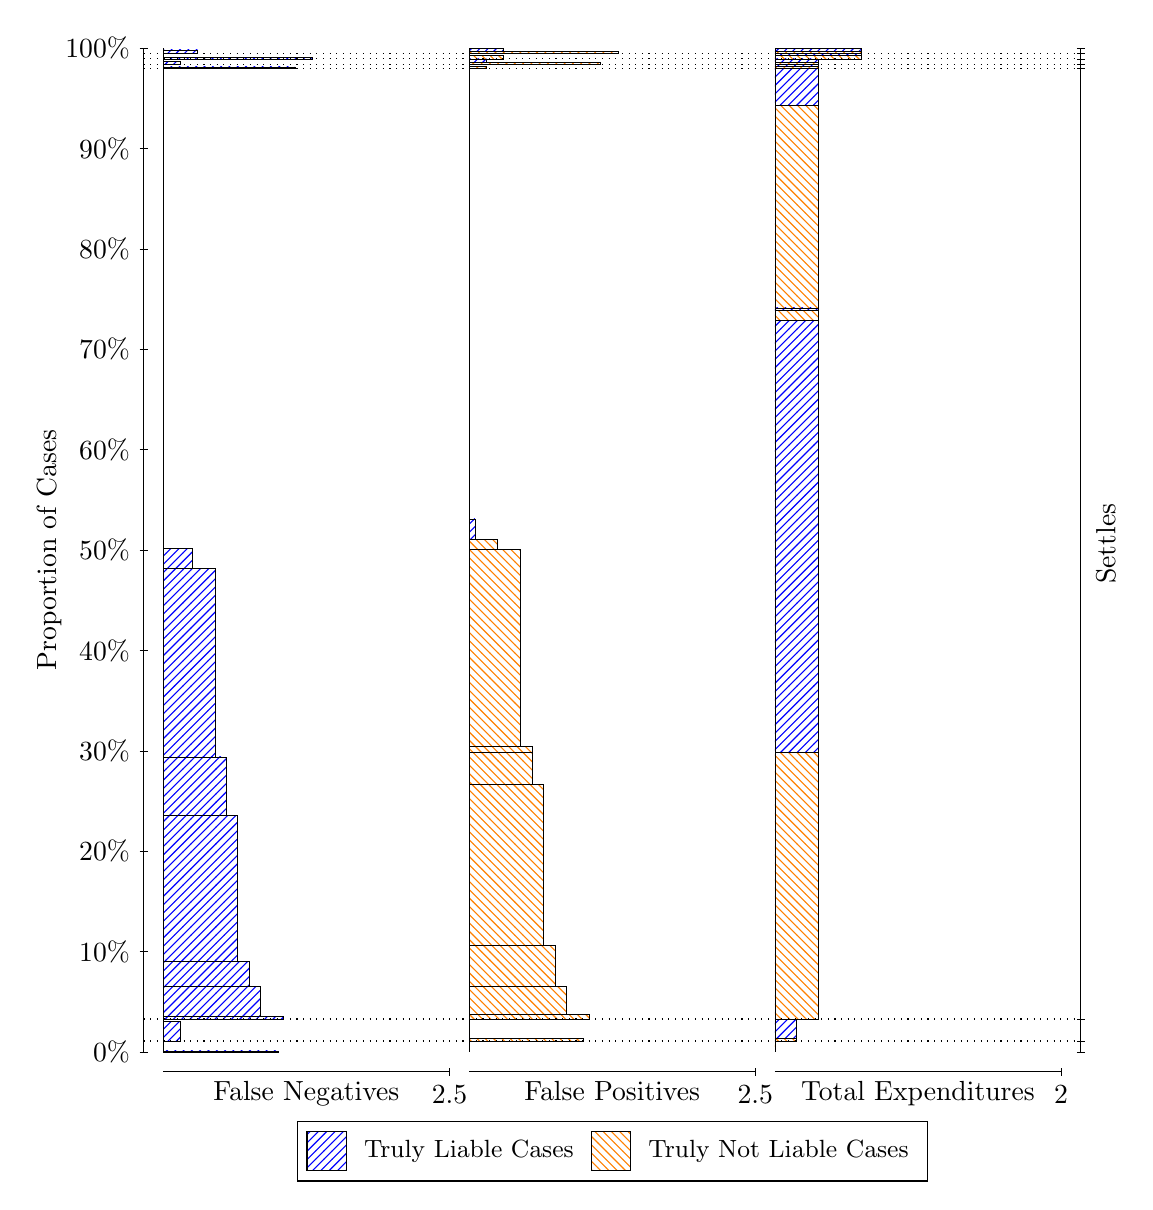
\begin{tikzpicture}
\draw[black, very thin] (1.5,1.75) -- (1.5,14.5);
\node[rotate=90, text=black, anchor=center] at (0.3, 8.125) {Proportion of Cases};
\draw[black, very thin] (1.45,1.75) -- (1.55,1.75);
\node[text=black, anchor=east] at (1.45, 1.75) {0\%};
\draw[black, very thin] (1.45,3.025) -- (1.55,3.025);
\node[text=black, anchor=east] at (1.45, 3.025) {10\%};
\draw[black, very thin] (1.45,4.3) -- (1.55,4.3);
\node[text=black, anchor=east] at (1.45, 4.3) {20\%};
\draw[black, very thin] (1.45,5.575) -- (1.55,5.575);
\node[text=black, anchor=east] at (1.45, 5.575) {30\%};
\draw[black, very thin] (1.45,6.85) -- (1.55,6.85);
\node[text=black, anchor=east] at (1.45, 6.85) {40\%};
\draw[black, very thin] (1.45,8.125) -- (1.55,8.125);
\node[text=black, anchor=east] at (1.45, 8.125) {50\%};
\draw[black, very thin] (1.45,9.4) -- (1.55,9.4);
\node[text=black, anchor=east] at (1.45, 9.4) {60\%};
\draw[black, very thin] (1.45,10.675) -- (1.55,10.675);
\node[text=black, anchor=east] at (1.45, 10.675) {70\%};
\draw[black, very thin] (1.45,11.95) -- (1.55,11.95);
\node[text=black, anchor=east] at (1.45, 11.95) {80\%};
\draw[black, very thin] (1.45,13.225) -- (1.55,13.225);
\node[text=black, anchor=east] at (1.45, 13.225) {90\%};
\draw[black, very thin] (1.45,14.5) -- (1.55,14.5);
\node[text=black, anchor=east] at (1.45, 14.5) {100\%};

\draw[black, very thin] (13.4,1.75) -- (13.4,14.5);
\draw[black, very thin] (13.35,1.75) -- (13.45,1.75);
\node[anchor=west] at (13.35, 1.75) {};
\draw[black, very thin] (13.35,1.8896) -- (13.45,1.8896);
\node[anchor=west] at (13.35, 1.8896) {};
\draw[black, very thin] (13.35,2.1686) -- (13.45,2.1686);
\node[anchor=west] at (13.35, 2.1686) {};
\draw[black, very thin] (13.35,14.241) -- (13.45,14.241);
\node[anchor=west] at (13.35, 14.241) {};
\draw[black, very thin] (13.35,14.288) -- (13.45,14.288);
\node[anchor=west] at (13.35, 14.288) {};
\draw[black, very thin] (13.35,14.362) -- (13.45,14.362);
\node[anchor=west] at (13.35, 14.362) {};
\draw[black, very thin] (13.35,14.432) -- (13.45,14.432);
\node[anchor=west] at (13.35, 14.432) {};
\draw[black, very thin] (13.35,14.5) -- (13.45,14.5);
\node[anchor=west] at (13.35, 14.5) {};

\draw[black, very thin, pattern color=blue, pattern=north east lines] (1.75,1.75) rectangle (3.2033,1.7647);
\draw[black, very thin, pattern color=orange, pattern=north west lines] (1.75,1.7647) rectangle (1.75,1.8896);
\draw[black, very thin, pattern color=blue, pattern=north east lines] (1.75,1.8896) rectangle (1.968,2.1393);
\draw[black, very thin, pattern color=orange, pattern=north west lines] (1.75,2.1393) rectangle (1.75,2.1686);
\draw[black, very thin, pattern color=blue, pattern=north east lines] (1.75,2.1686) rectangle (3.276,2.1972);
\draw[black, very thin, pattern color=blue, pattern=north east lines] (1.75,2.1972) rectangle (2.9853,2.581);
\draw[black, very thin, pattern color=blue, pattern=north east lines] (1.75,2.581) rectangle (2.84,2.8957);
\draw[black, very thin, pattern color=blue, pattern=north east lines] (1.75,2.8957) rectangle (2.6947,4.7514);
\draw[black, very thin, pattern color=blue, pattern=north east lines] (1.75,4.7514) rectangle (2.5493,5.4975);
\draw[black, very thin, pattern color=blue, pattern=north east lines] (1.75,5.4975) rectangle (2.404,7.8885);
\draw[black, very thin, pattern color=blue, pattern=north east lines] (1.75,7.8885) rectangle (2.1133,8.1488);
\draw[black, very thin, pattern color=orange, pattern=north west lines] (1.75,8.1488) rectangle (1.75,14.241);
\draw[black, very thin, pattern color=blue, pattern=north east lines] (1.75,14.241) rectangle (3.4213,14.261);
\draw[black, very thin, pattern color=orange, pattern=north west lines] (1.75,14.261) rectangle (1.75,14.288);
\draw[black, very thin, pattern color=blue, pattern=north east lines] (1.75,14.288) rectangle (1.968,14.331);
\draw[black, very thin, pattern color=orange, pattern=north west lines] (1.75,14.331) rectangle (1.75,14.362);
\draw[black, very thin, pattern color=blue, pattern=north east lines] (1.75,14.362) rectangle (3.6393,14.386);
\draw[black, very thin, pattern color=orange, pattern=north west lines] (1.75,14.386) rectangle (1.75,14.432);
\draw[black, very thin, pattern color=blue, pattern=north east lines] (1.75,14.432) rectangle (2.186,14.476);
\draw[black, very thin, pattern color=orange, pattern=north west lines] (1.75,14.476) rectangle (1.75,14.5);
\draw[black, very thin, pattern color=orange, pattern=north west lines] (5.6333,1.75) rectangle (5.6333,1.8749);
\draw[black, very thin, pattern color=blue, pattern=north east lines] (5.6333,1.8749) rectangle (5.6333,1.8896);
\draw[black, very thin, pattern color=orange, pattern=north west lines] (5.6333,1.8896) rectangle (7.0867,1.9189);
\draw[black, very thin, pattern color=blue, pattern=north east lines] (5.6333,1.9189) rectangle (5.6333,2.1686);
\draw[black, very thin, pattern color=orange, pattern=north west lines] (5.6333,2.1686) rectangle (7.1593,2.2257);
\draw[black, very thin, pattern color=orange, pattern=north west lines] (5.6333,2.2257) rectangle (6.8687,2.5847);
\draw[black, very thin, pattern color=orange, pattern=north west lines] (5.6333,2.5847) rectangle (6.7233,3.0988);
\draw[black, very thin, pattern color=orange, pattern=north west lines] (5.6333,3.0988) rectangle (6.578,5.1526);
\draw[black, very thin, pattern color=orange, pattern=north west lines] (5.6333,5.1526) rectangle (6.4327,5.5586);
\draw[black, very thin, pattern color=orange, pattern=north west lines] (5.6333,5.5586) rectangle (6.4327,5.6272);
\draw[black, very thin, pattern color=orange, pattern=north west lines] (5.6333,5.6272) rectangle (6.2873,8.1311);
\draw[black, very thin, pattern color=orange, pattern=north west lines] (5.6333,8.1311) rectangle (5.9967,8.2612);
\draw[black, very thin, pattern color=blue, pattern=north east lines] (5.6333,8.2612) rectangle (5.706,8.5215);
\draw[black, very thin, pattern color=blue, pattern=north east lines] (5.6333,8.5215) rectangle (5.6333,14.241);
\draw[black, very thin, pattern color=orange, pattern=north west lines] (5.6333,14.241) rectangle (5.8513,14.269);
\draw[black, very thin, pattern color=blue, pattern=north east lines] (5.6333,14.269) rectangle (5.6333,14.288);
\draw[black, very thin, pattern color=orange, pattern=north west lines] (5.6333,14.288) rectangle (7.3047,14.319);
\draw[black, very thin, pattern color=blue, pattern=north east lines] (5.6333,14.319) rectangle (5.8513,14.362);
\draw[black, very thin, pattern color=orange, pattern=north west lines] (5.6333,14.362) rectangle (6.0693,14.408);
\draw[black, very thin, pattern color=blue, pattern=north east lines] (5.6333,14.408) rectangle (5.6333,14.432);
\draw[black, very thin, pattern color=orange, pattern=north west lines] (5.6333,14.432) rectangle (7.5227,14.456);
\draw[black, very thin, pattern color=blue, pattern=north east lines] (5.6333,14.456) rectangle (6.0693,14.5);
\draw[black, very thin, pattern color=orange, pattern=north west lines] (9.5167,1.75) rectangle (9.5167,1.8749);
\draw[black, very thin, pattern color=blue, pattern=north east lines] (9.5167,1.8749) rectangle (9.5167,1.8896);
\draw[black, very thin, pattern color=orange, pattern=north west lines] (9.5167,1.8896) rectangle (9.7892,1.9189);
\draw[black, very thin, pattern color=blue, pattern=north east lines] (9.5167,1.9189) rectangle (9.7892,2.1686);
\draw[black, very thin, pattern color=orange, pattern=north west lines] (9.5167,2.1686) rectangle (10.062,5.5586);
\draw[black, very thin, pattern color=blue, pattern=north east lines] (9.5167,5.5586) rectangle (10.062,11.042);
\draw[black, very thin, pattern color=orange, pattern=north west lines] (9.5167,11.042) rectangle (10.062,11.172);
\draw[black, very thin, pattern color=blue, pattern=north east lines] (9.5167,11.172) rectangle (10.062,11.201);
\draw[black, very thin, pattern color=orange, pattern=north west lines] (9.5167,11.201) rectangle (10.062,13.773);
\draw[black, very thin, pattern color=blue, pattern=north east lines] (9.5167,13.773) rectangle (10.062,14.241);
\draw[black, very thin, pattern color=orange, pattern=north west lines] (9.5167,14.241) rectangle (10.062,14.269);
\draw[black, very thin, pattern color=blue, pattern=north east lines] (9.5167,14.269) rectangle (10.062,14.288);
\draw[black, very thin, pattern color=orange, pattern=north west lines] (9.5167,14.288) rectangle (10.062,14.319);
\draw[black, very thin, pattern color=blue, pattern=north east lines] (9.5167,14.319) rectangle (10.062,14.362);
\draw[black, very thin, pattern color=orange, pattern=north west lines] (9.5167,14.362) rectangle (10.607,14.408);
\draw[black, very thin, pattern color=blue, pattern=north east lines] (9.5167,14.408) rectangle (10.607,14.432);
\draw[black, very thin, pattern color=orange, pattern=north west lines] (9.5167,14.432) rectangle (10.607,14.456);
\draw[black, very thin, pattern color=blue, pattern=north east lines] (9.5167,14.456) rectangle (10.607,14.5);
\draw[black, dotted] (1.5,1.8896) -- (13.4,1.8896);
\draw[black, dotted] (1.5,2.1686) -- (13.4,2.1686);
\draw[black, dotted] (1.5,14.241) -- (13.4,14.241);
\draw[black, dotted] (1.5,14.288) -- (13.4,14.288);
\draw[black, dotted] (1.5,14.362) -- (13.4,14.362);
\draw[black, dotted] (1.5,14.432) -- (13.4,14.432);
\draw[black, very thin] (1.75,1.5) -- (5.3833,1.5);
\node[text=black, anchor=north] at (3.5667, 1.5) {False Negatives};
\draw[black, very thin] (5.3833,1.45) -- (5.3833,1.55);
\node[text=black, anchor=north] at (5.3833, 1.45) {2.5};

\draw[black, very thin] (5.6333,1.5) -- (9.2667,1.5);
\node[text=black, anchor=north] at (7.45, 1.5) {False Positives};
\draw[black, very thin] (9.2667,1.45) -- (9.2667,1.55);
\node[text=black, anchor=north] at (9.2667, 1.45) {2.5};

\draw[black, very thin] (9.5167,1.5) -- (13.15,1.5);
\node[text=black, anchor=north] at (11.333, 1.5) {Total Expenditures};
\draw[black, very thin] (13.15,1.45) -- (13.15,1.55);
\node[text=black, anchor=north] at (13.15, 1.45) {2};



\node[text=black, centered, rotate=90] at (13.72, 8.205) {Settles};





\draw (7.449999999999999,1.5) node[draw=none] (baseCoordinate) {};
\begin{scope}[align=center]
        \matrix[scale=0.5, draw=black, below=0.5cm of baseCoordinate, nodes={draw}, column sep=0.1cm]{
            \node[rectangle, draw, minimum width=0.5cm, minimum height=0.5cm, pattern color=blue, pattern=north east lines] {}; &
            \node[draw=none, font=\small, text=black] (B) {Truly Liable Cases}; &
            \node[rectangle, draw, minimum width=0.5cm, minimum height=0.5cm, pattern color=orange, pattern=north west lines] {}; &
            \node[draw=none, font=\small, text=black] (B) {Truly Not Liable Cases}; \\
            };
\end{scope}

\end{tikzpicture}
\end{document}